\documentclass[aspectratio=169]{beamer}
\usetheme{simple}
\usepackage{lmodern}
\usepackage[scale=2]{ccicons}
\usepackage{booktabs}
\usepackage{caption}
\usepackage{subcaption}
\usepackage{graphicx}
\usepackage{amsmath}
\usepackage{amssymb}
\usepackage{epstopdf}
\usepackage{enumitem} %Comment out enumitem if you want round ("default") bullet points
\useinnertheme{rectangles} % Uncomment this (and comment out enumitem) if you want to use different bullet points
\usepackage{hyperref}
\usepackage[style=numeric]{biblatex}
\usepackage{listings}

\renewcommand{\rmdefault}{cmr} % Resets the default roman font to CM
\renewcommand{\sfdefault}{cmss} % Resets the default sans serif font to CM
\renewcommand{\ttdefault}{cmtt} % Resets the default typewriter font to CM

% TODO: 
%   position adjustement
%   change colours
%       

% Watermark background (simple theme)

\logo{%
    
\includegraphics[height=0.7cm,keepaspectratio]{image/iade_ipca_logo.png}~%
    \vspace{230pt}
}

\setbeamercolor{footline}{fg=white,bg=blue} % Set the footer foreground and background colors
\setbeamercolor{navigation symbols dimmed}{fg=gray} % Optional: Set dimmed navigation symbols color
\setbeamercolor{navigation symbols}{fg=white} % Set navigation symbols color

\setbeamertemplate{navigation symbols}{} % Disable navigation symbols

\setbeamertemplate{footline}
{
  \leavevmode%
  \hbox{%
  \begin{beamercolorbox}[wd=\paperwidth,ht=2.25ex,dp=1ex,center]{footline}%
    \hfill \insertsection\hspace*{2ex}
    \hfill \insertsubsection\hspace*{2ex}
    % Now just some space 
    \hfill \hspace*{2ex}
    \hfill \hspace*{2ex}
    \hfill \hspace*{2ex}
    \hfill \hspace*{2ex}
    \hfill \insertframenumber{} / \inserttotalframenumber\hspace*{2ex} 
  \end{beamercolorbox}%
  }%
  \vskip0pt%
}


\title{Spiking Neural Networks \\Sound Detection and Classification}
\subtitle{}
\date{\today}
\author{COURREGE Téo\\GANDEEL Loaï}
\institute{\url{https://github.com/LGPolytech/Project\_S9}}

\begin{document}

\maketitle

\section{Introduction}

\begin{frame}
  \frametitle{Introduction}
  \tableofcontents

\end{frame}


\section{Rappels}

\subsection{Spikes et Spike encoding}
\begin{frame}
  \frametitle{Spike ou impulsions électriques}

  \begin{itemize}
    \item Impulsion électrique de courte durée ($I_{in}$)
    \item Modèle de communication entre neurones
    \item Permet de transmettre de l'information
  \end{itemize}

  \begin{center}
    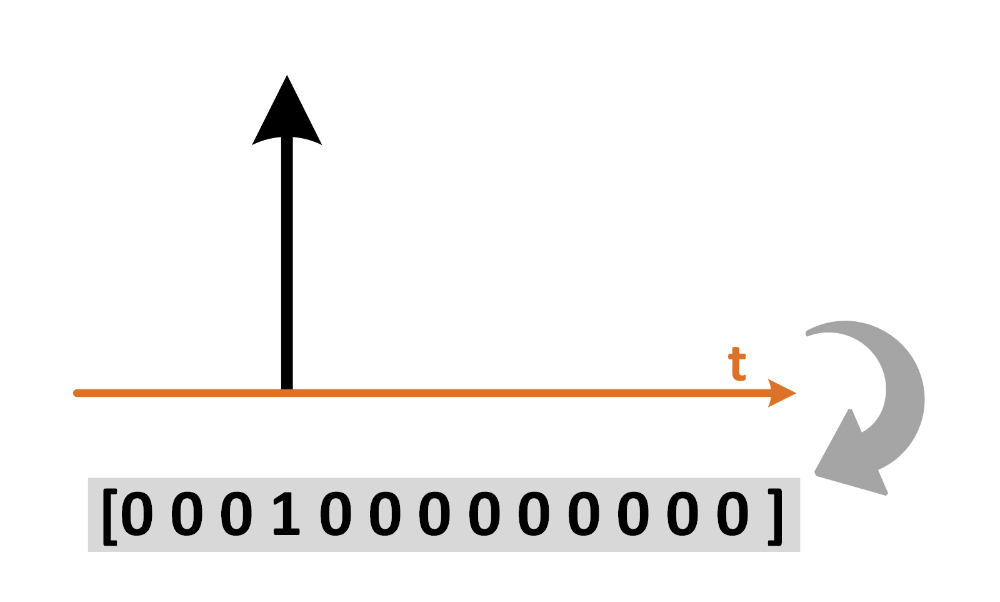
\includegraphics[width=0.6\textwidth]{image/spikeboy.png}
  \end{center}

\end{frame}

\begin{frame}
  \frametitle{Encodage de l'information en spikes}
  \begin{columns}
    \begin{column}{0.5\textwidth}
      \begin{itemize}
        \item Manière de représenter l'information
        \item Approximation de l'information par des impulsions électriques
        \item Variable temporelle ou fréquentielle
        \item Encodage temporel, fréquentiel, ou mixte
      \end{itemize}
    \end{column}
    \begin{column}{0.5\textwidth}
      \begin{center}
        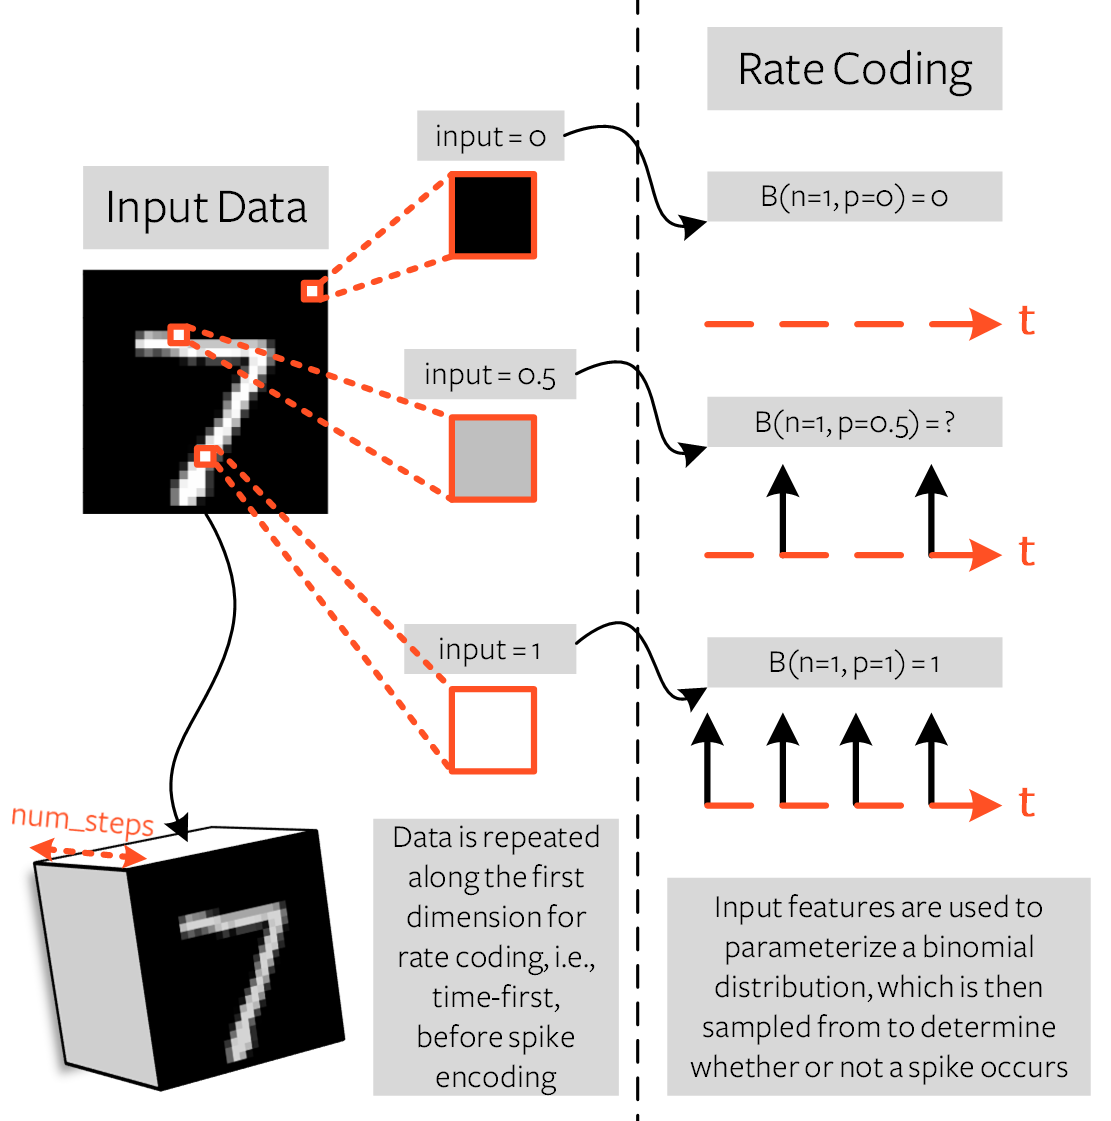
\includegraphics[width=0.8\textwidth]{image/1_2_3_spikeconv.png}
      \end{center}
    \end{column}
  \end{columns}
\end{frame}

% Gif de l'encodage temporel
\begin{frame}
  \frametitle{Exemple avec MNIST}

\end{frame}

\subsection{Neurones spikant}

\begin{frame}
  \frametitle{Modèle Leaky Integrate and Fire (LIF)}
  \begin{columns}
    \begin{column}{0.5\textwidth}
      $$\begin{aligned}
           & U[t+1] = \underbrace{\beta U[t]}_\text{decay} + \underbrace{WX[t+1]}_\text{input} - \underbrace{\beta S[t]U_{\rm thr}}_\text{soft reset} \\
           & S[t] =
          \begin{cases}
            1, & \text{if } U[t] > U_{\rm thr} \\
            0, & \text{otherwise}
          \end{cases}\end{aligned}$$
      \begin{itemize}
        \item $U$ : Potentiel de membrane
        \item $W$ : Poids du réseau
        \item $X$ : Entrée du réseau (des spikes)
        \item $S$ : Fonction de spike
        \item $\beta \in ]0, 1[$ : Facteur de décharge
      \end{itemize}
    \end{column}
    \begin{column}{0.5\textwidth}
      \begin{center}
        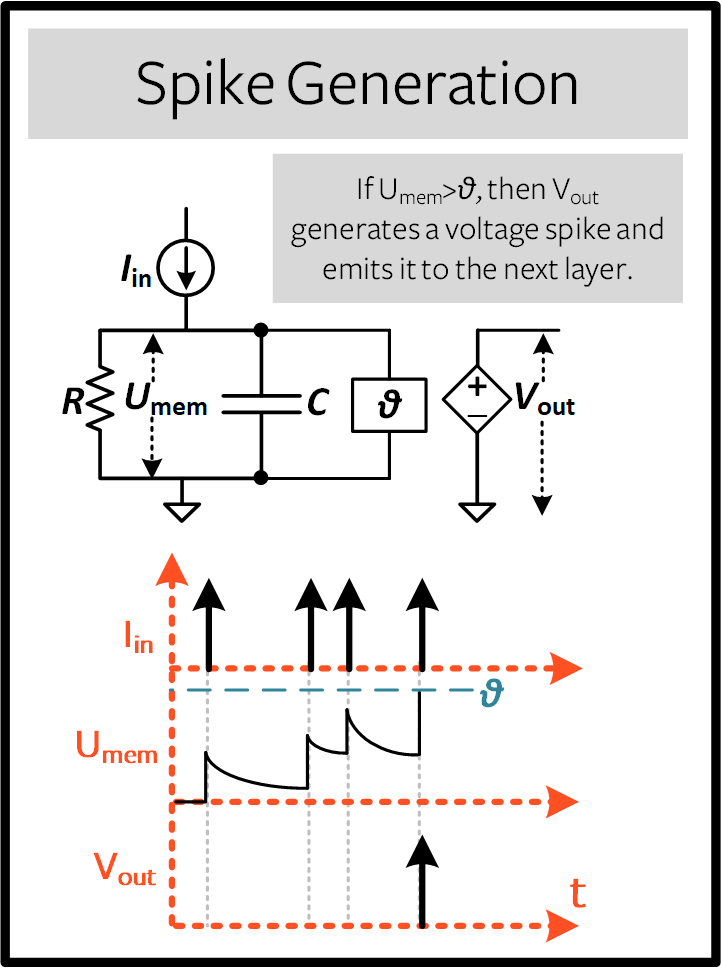
\includegraphics[width=0.7\textwidth]{image/2_4_spiking.png}
      \end{center}

    \end{column}
  \end{columns}
\end{frame}

\begin{frame}
  \frametitle{LiF : Illustration}
  

\end{frame}

\subsection{Réseau de neurones spikants}

\begin{frame}
  \frametitle{Définition d'un réseau de neurones}


\end{frame}

\begin{frame}
  \frametitle{Convolutional Spiking Neural Networks}

  \begin{center}
    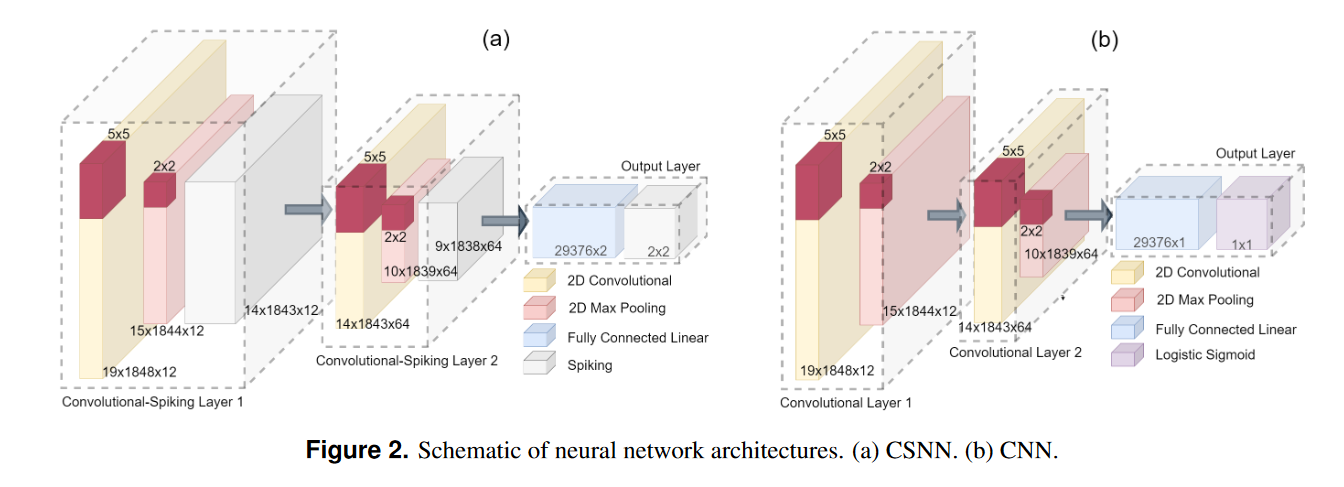
\includegraphics[width=\textwidth]{image/Convo.png}
  \end{center}

\end{frame}

\section{SNN - Behind the scene}

\subsection{Entrainer un SNN}

\begin{frame}
  \frametitle{Le problème de la backpropagation}
  Expression générale de la backpropagation :
  $$
    \begin{aligned}
       & \frac{\partial \mathcal{L}}{\partial W} =
      \frac{\partial \mathcal{L}}{\partial S}
      \underbrace{\frac{\partial S}{\partial U}}_{\{0, \infty\}}
      \frac{\partial U}{\partial I}
      \frac{\partial I}{\partial W}
    \end{aligned}
  $$

  \begin{itemize}
    \item $\mathcal{L}$ : la loss function
    \item $W$ : les poids du réseau
    \item $S$ : fonction qui génére un spike
    \item $U$ : Le potentiel de la membrane
    \item $I = WX$ : L'entrée du réseau (input)
  \end{itemize}

\end{frame}

\subsection{Dead Neuron Problem}

\begin{frame}
  \frametitle{Un challenge, plusieurs solutions}

  Le challenge : La non différentiabilité de sorties spikantes (dead neuron problem)

  Les solutions :
  \begin{itemize}
    \item Shadow training :
          Transformer un ANN en SNN
    \item Surrogate Gradient (ou dérivée approchée)
          $$\begin{aligned}
              \tilde{S}(U) & \approx \frac{1}{1 + e^{-(U - U_{thr})}}       \\                        \\
              \tilde{S}(U) & \approx \frac{U}{1 + k \lvert U \rvert}
            \end{aligned}$$
  \end{itemize}

\end{frame}

\subsection{Surrogate gradient}

\begin{frame}
  \scriptsize{Entraînement : Gradient Surrogate}

  \begin{block}{Gradient général}
    Le gradient de la loss function générale $\mathcal{L}$ par rapport aux poids $W$ est donné par :
    \[
    \color{blue} \frac{\partial \mathcal{L}}{\partial W} = \sum_t \sum_{s\leq t} \frac{\partial\mathcal{L}[t]}{\partial W[s]}
    \]
  \end{block}

  \vspace{1em} % Ajoute un espace vertical

  \begin{block}{Chain rule}
    \[
    \color{blue} \frac{\partial \mathcal{L}[t]}{\partial W[t-1]} = \frac{\partial \mathcal{L}[t]}{\partial S[t]} \frac{\partial \tilde{S}[t]}{\partial U[t]} \frac{\partial U[t]}{\partial U[t-1]} \frac{\partial U[t-1]}{\partial I[t-1]} \frac{\partial I[t-1]}{\partial W[t-1]}
    \]
  \end{block}

  \vspace{1em} % Ajoute un espace vertical

  \begin{block}{Influence du poids précédent}
    \[
    \color{blue} \frac{\partial \mathcal{L}[t]}{\partial W[t-1]} = \frac{\partial \mathcal{L}[t]}{\partial S[t]} \frac{\partial \tilde{S}[t]}{\partial U[t]} \cdot \beta \cdot X[t-1]
    \]
  \end{block}
\end{frame}



\begin{frame}
  \frametitle{Entrainement : Surrogate gradient}

  \begin{center}
    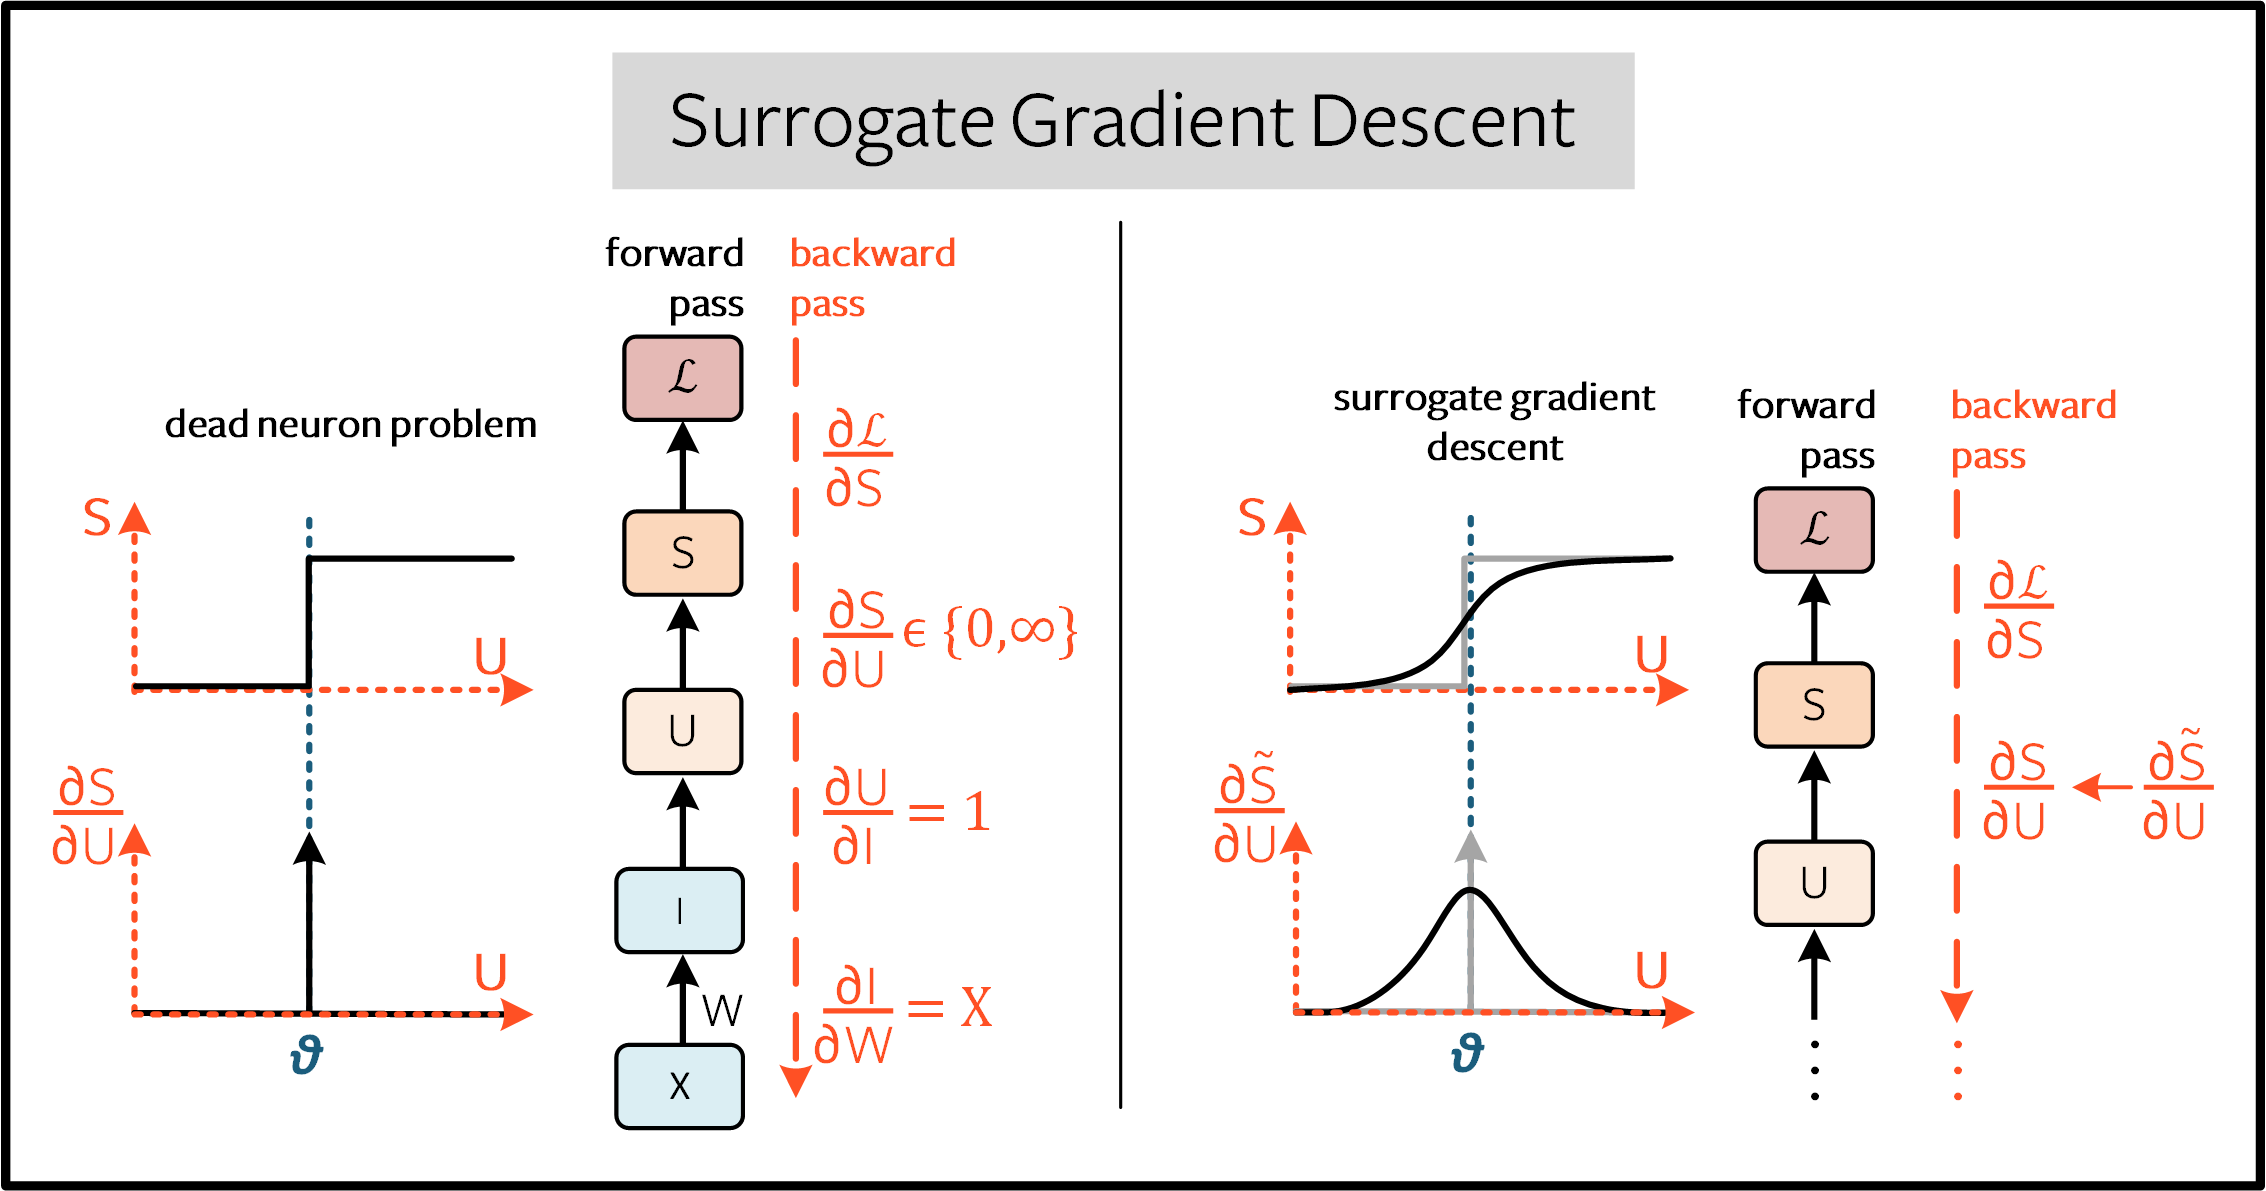
\includegraphics[width=0.8\textwidth]{image/surrogate.png}
  \end{center}
\end{frame}

\begin{frame}
  \frametitle{Entrainement}
  \begin{columns}
    \begin{column}{0.5\textwidth}
      \begin{center}
        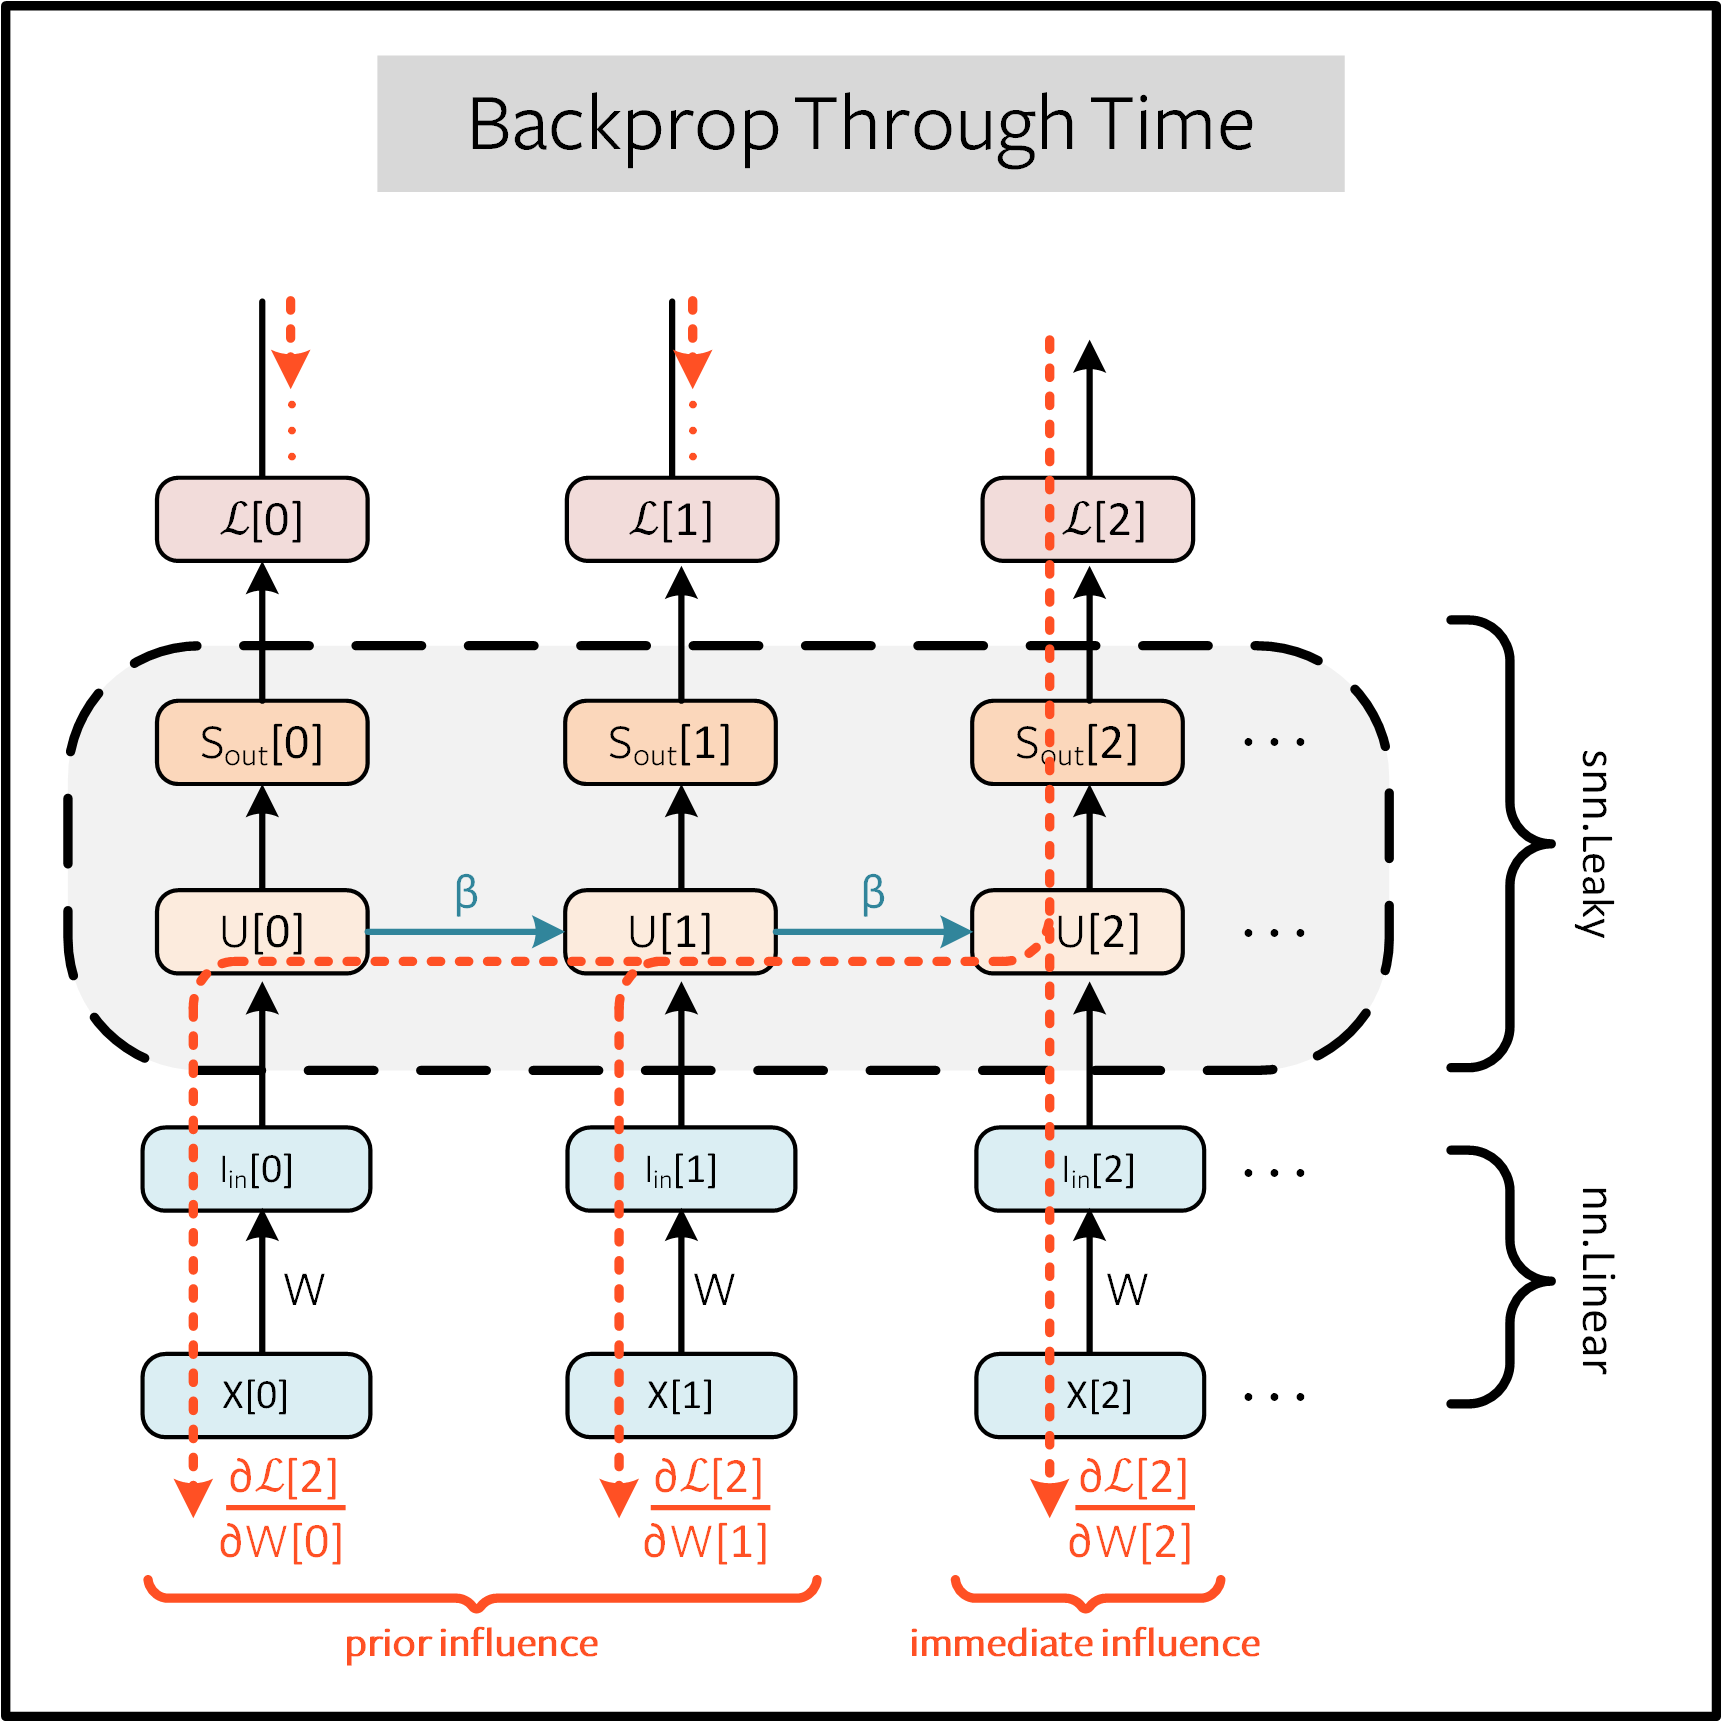
\includegraphics[width=0.9\textwidth]{image/bptt.png}
      \end{center}
    \end{column}
    \begin{column}{0.5\textwidth}
      \begin{itemize}
        \item Les spikes sont des événements asynchrones
        \item Les événements temporels à générer
        \item Les poids à ajuster
        \item Tout cela mutliplié par le nombre de neurones et la complexité des données
      \end{itemize}
    \end{column}
  \end{columns}

\end{frame}

\section{Classification et résultats}

\subsection{MNIST}

\begin{frame}
  \frametitle{Résultats sur MNIST}


\end{frame}

\subsection{Dataset pour la classification sonore}

\begin{frame}
  \frametitle{Dataset pour la classification sonore}

\end{frame}

\begin{frame}
  \frametitle{Du signal audio aux MFCC}
  \scriptsize{ % Réduit encore plus la taille de la police pour tout le contenu de la diapositive

  \begin{block}{\color{gray} STFT}
    \[
    \color{blue} \left\{ x[ n ] \right\} \equiv X(m,\omega) = \sum_{n=-\infty}^{\infty} x[n]w[n-m]\mathrm{e}^{-j \omega n}
    \]
  \end{block}

  \vspace{0.5em} % Réduit l'espace vertical

  \begin{block}{\color{gray} Echelle Mel}
    \[
    \color{blue} m = 2595 \log_{10}\left(1 + \frac{f}{700}\right)
    \]
  \end{block}

  \vspace{0.5em} % Réduit l'espace vertical

  \begin{block}{\color{gray} DCT}
    \[
    \color{blue} S_{u,v} = \sum_{m = 0}^{M- 1} \sum_{n = 0}^{N- 1} s(m, n)\mathrm e^{-2\mathrm i\pi \left ( \frac{um}M+ \frac{vn}N\right )}
    \]
  \end{block}
  } % Fin de \scriptsize
\end{frame}
\begin{frame}
  \frametitle{Du signal audio vers le MFCC}

  

\end{frame}

\subsection{Résultats sur notre dataset}

\begin{frame}
  \frametitle{Résultats sur notre dataset}
  
  Guitare 
\end{frame}

\begin{frame}
  \frametitle{Conclusion}

  \begin{itemize}
    \item Le fonctionnement des SNNs
    \item Les challenges de l'entrainement
    \item Les résultats
    \item Malgrès la durée d'entrainement, sparsité et efficacité
    \begin{itemize}
      \item Utiles pour les systèmes embarqués
    \end{itemize}
    \item Applications intéressantes :
          \begin{itemize}
            \item Détection de sons
            \item Classification en temps réel
          \end{itemize}
    
  \end{itemize}
\end{frame}

\end{document}